\chapter{Perancangan}
\label{chap:perancangan}

Pada bab ini akan dibahas mengenai perancangan permainan yang dibangun. Perancangan akan dilakukan meliputi perancangan diagram \textit{sequence}, perancangan diagram \textit{state}, perancangan diagram kelas, dan perancangan tampilan antarmuka.

\section{Rancangan Diagram \textit{Sequence}}
Pada bagian ini akan ditunjukan dan dijelaskan diagram \textit{sequence} Open Source Snake 360. Diagram \textit{sequence} yang dibuat adalah memuat labirin. 

\begin{figure}[H]
	\centering  
	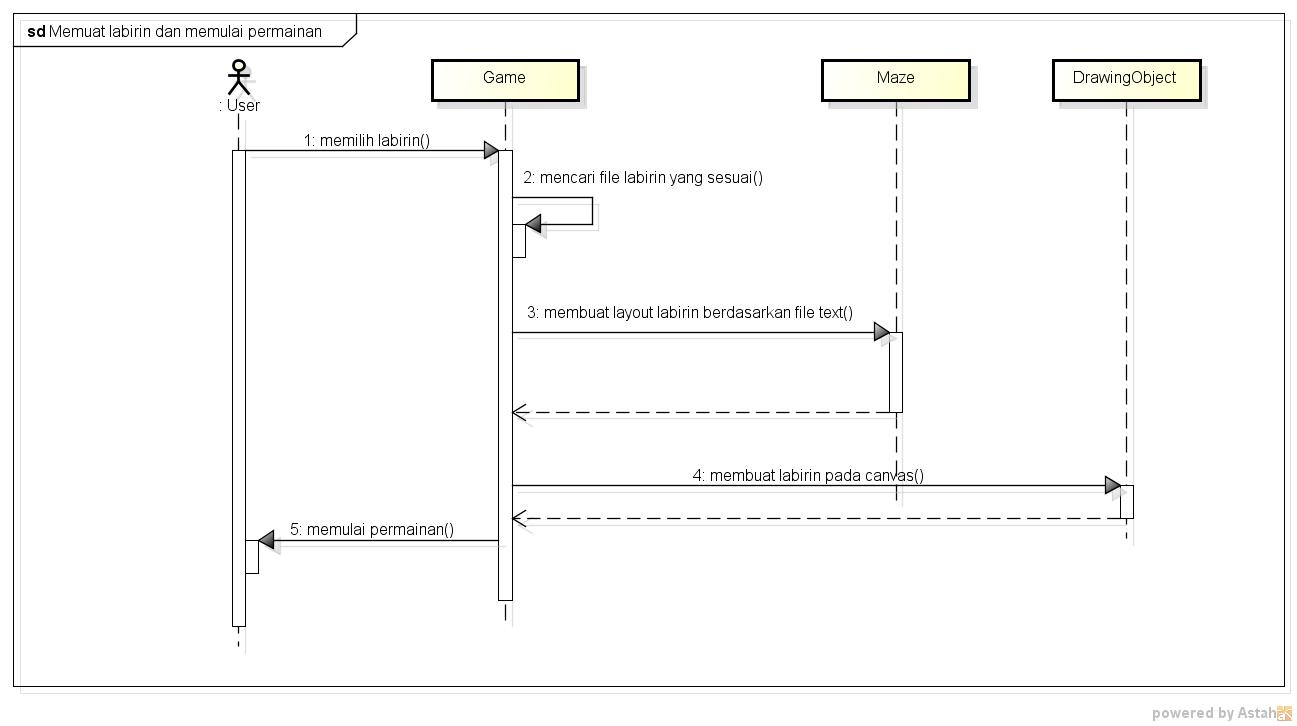
\includegraphics[scale=0.3]{sequenceLoad}  
	\caption[Diagram \textit{sequence} untuk memuat labirin]{Diagram \textit{sequence} untuk memuat labirin}
	\label{fig:sequenceLoad} 
\end{figure}

Pada Gambar~\ref{fig:sequenceLoad}, pemain memulai bermain dengan memilih labirin. Berikut adalah penjelasan dari Gambar~\ref{fig:sequenceLoad}:

\begin{enumerate}
	\item Pemain memilih labirin. 
	\item Kelas \textit{Game} akan menerima input dari pemain dan mencari \textit{file} labirin yang sesuai dengan yang pemain pilih di folder labirin. \textit{File} labirin merupakan file teks.
	\item Jika \textit{file} ditemukan, maka kelas \textit{Game} akan memanggil \textit{method} kelas \textit{Maze} untuk membuat labirin yang sesuai dengan isi \textit{file} labirin. 
	\item Setelah labirin selesai dibuat, kelas Game akan memanggil \textit{method} kelas \textit{DrawingObject} untuk menggambar labirin.
	\item Jika labirin sudah selesai digambar, kelas Game akan memulai permainan.
\end{enumerate}

\section{Rancangan Diagram \textit{State}}
Pada bagian ini akan ditunjukan diagram \textit{state} pada Open Source Snake 360. Diagram \textit{state} yang dibuat adalah proses bermain mulai dari awal sampai akhir permainan. Diagram \textit{state} dapat dilihat pada Gambar~\ref{fig:stateDiagram}.

\begin{figure}[H]
	\centering  
	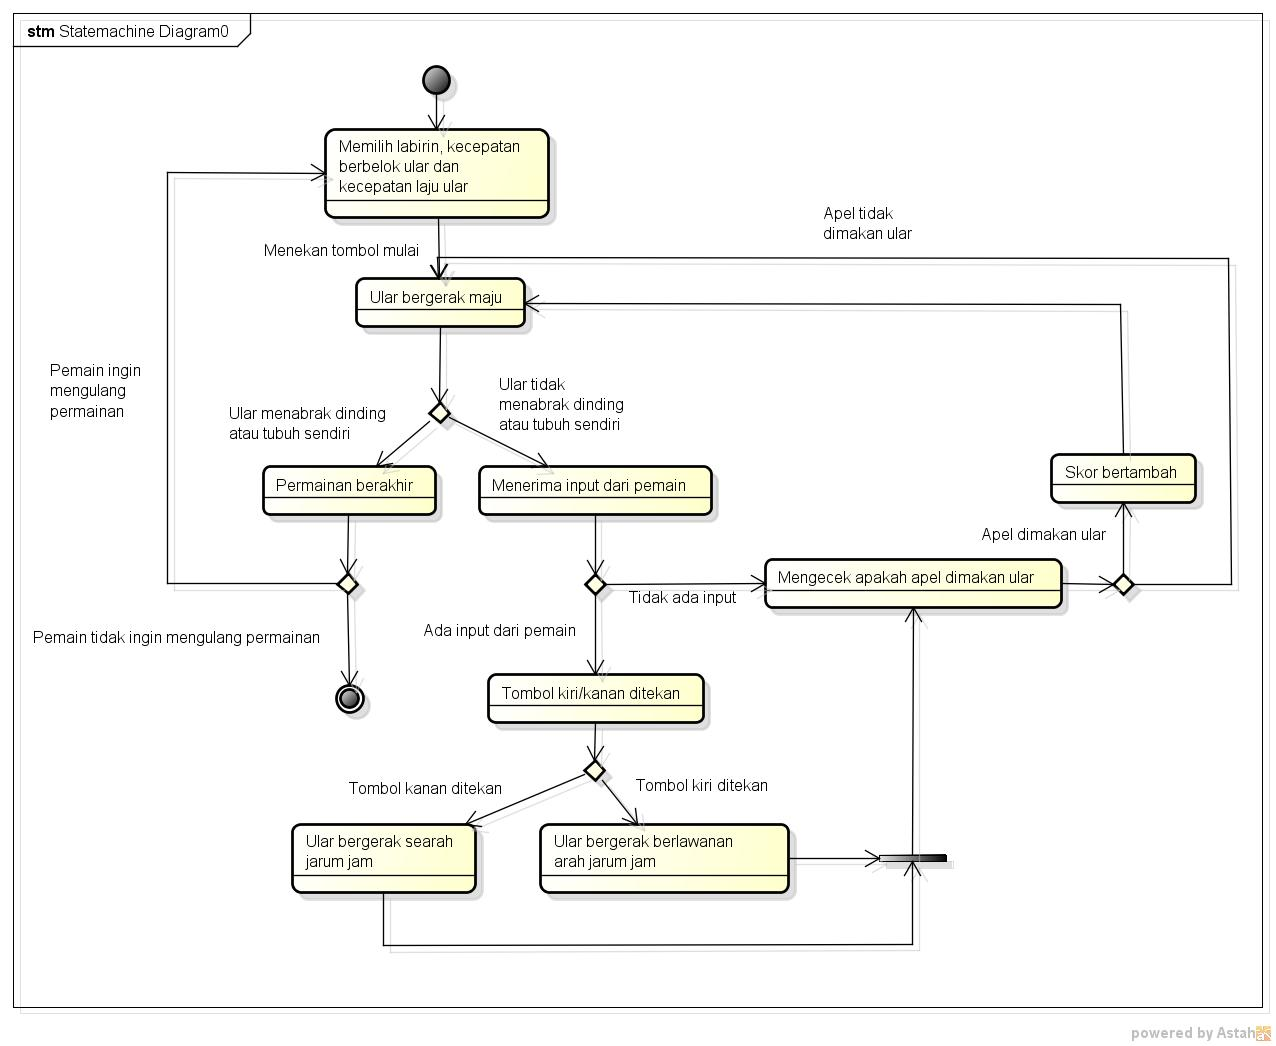
\includegraphics[scale=0.4]{stateDiagram}  
	\caption[Diagram state proses bermain dari Open Source \textit{Snake} 360]{Diagram state proses bermain dari Open Source \textit{Snake} 360}
	\label{fig:stateDiagram} 
\end{figure}

\section{Rancangan Diagram Kelas Rinci}
Pada bagian ini akan ditunjukan dan dijelaskan diagram kelas dari \textit{Open Source Snake 360} secara lengkap. Diagram kelas dapat dilihat pada Gambar~\ref{fig:classDiagramComplete}.

\begin{figure}[H]
	\centering  
	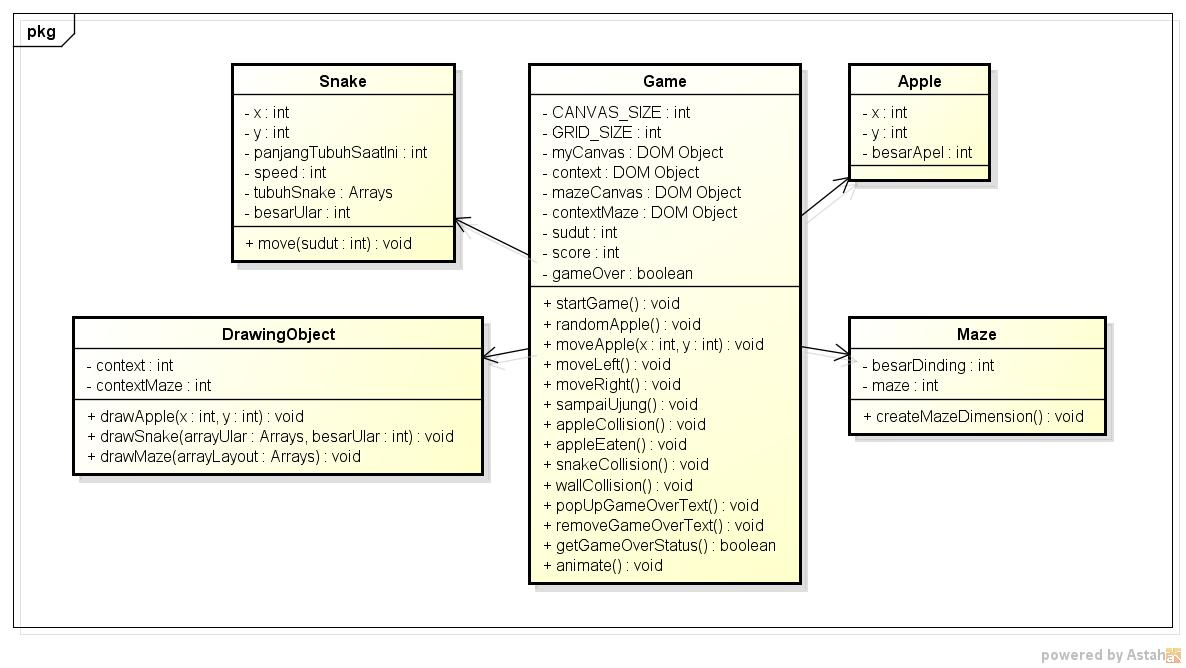
\includegraphics[scale=0.4]{classDiagramComplete}  
	\caption[Diagram class rinci dari Open Source \textit{Snake} 360]{Diagram kelas rinci dari Open Source \textit{Snake} 360}
	\label{fig:classDiagramComplete} 
\end{figure}

\textbf{Deskripsi Kelas dan Method}\\

Pada bagian ini akan dijelaskan deskripsi kelas dan \textit{method-method} pada setiap kelas. Penjelasan kelas dan \textit{method} meliputi nama kelas, deskripsi \textit{method}, \textit{input} yang dibutuhkan, dan \textit{output} yang dihasilkan. 

\begin{enumerate}
	\item Kelas \textit{Game} \\
	Kelas \textit{Game} merupakan kelas utama dari permainan ini. Kelas ini mengatur jalannya permainan.
		
		\begin{itemize}
			\item Nama \textit{method} : \textit{startGame}\\
				  Deskripsi : memulai permainan\\
				  Input : tidak ada\\
				  Output : tidak ada\\
			\item Nama \textit{method} : \textit{randomApple}\\
				  Deskripsi : mengacak posisi apel\\
				  Input : tidak ada\\
				  Output : tidak ada\\
			\item Nama \textit{method} : \textit{moveApple}\\
				  Deskripsi : memindahkan posisi apel\\
				  Input : \textit{int} x, \textit{int} y
				  	\begin{itemize}
				  		\item x : koordinat x milik apel
				  		\item y : koordinat y milik apel
				  	\end{itemize}
				  Output : tidak ada\\
			\item Nama \textit{method} : \textit{moveLeft}\\
				  Deskripsi : membuat ular bergerak berlawanan arah jarum jam\\
				  Input : tidak ada\\
				  Output : tidak ada\\
			\item Nama \textit{method} : \textit{moveRight}\\
				  Deskripsi : membuat ular bergerak searah jarum jam\\
				  Input : tidak ada\\
				  Output : tidak ada\\
			\item Nama \textit{method} : sampaiUjung\\
				  Deskripsi : membuat ular akan muncul di sisi yang berlawanan ketika ular sudah mencapai ujung labirin\\
				  Input : tidak ada\\
				  Output : tidak ada\\
			\item Nama \textit{method} : \textit{appleColiision}\\
				  Deskripsi : mengecek tabrakan antara apel dengan kepala ular\\
				  Input : tidak ada\\
				  Output : tidak ada\\
			\item Nama \textit{method} : \textit{appleEaten}\\
				  Deskripsi : aksi yang dilakukan apabila ular sudah memakan apel\\
				  Input : tidak ada\\
				  Output : tidak ada\\
			\item Nama \textit{method} : \textit{snakeCollision}\\
				  Deskripsi : mengecek tabrakan antara kepala ular dengan tubuhnya sendiri\\
				  Input : tidak ada\\
				  Output : tidak ada\\
			\item Nama \textit{method} : \textit{wallCollision}\\
				  Deskripsi : mengecek tabrakan antara kepala ular dengan dinding labirin\\
				  Input : tidak ada\\
				  Output : tidak ada\\
			\item Nama \textit{method} : \textit{popUpGameOverText}\\
				  Deskripsi : memunculkan tulisan 'Game Over'\\
				  Input : tidak ada\\
				  Output : tidak ada\\
			\item Nama \textit{method} : \textit{removeGameOverText}\\
				  Deskripsi : menghilangkan tulisan 'Game Over'\\
				  Input : tidak ada\\
				  Output : tidak ada\\
			\item Nama \textit{method} : \textit{getGameOverStatus}\\
				  Deskripsi : mendapatkan status gameOver\\
				  Input : tidak ada\\
				  Output : \textit{boolean gameOver}
				  	\begin{itemize}
				  		\item \textit{gameOver} : status apabila permainan sudah berakhir atau belum
				  	\end{itemize}
			\item Nama \textit{method} : \textit{animate}\\
				  Deskripsi : membuat animasi dari setiap objek\\
				  Input : tidak ada\\
				  Output : tidak ada
			\item Nama \textit{method} : \textit{changeLevel}\\
				  Deskripsi : mengubah jumlah labirin pada menu utama \\
				  Input : \textit{int} levels
				  	\begin{itemize}
				  		\item \textit{levels} : jumlah \textit{labirin} pada server
				  	\end{itemize}
				  Output : tidak ada
			\item Nama \textit{method} : \textit{loadMaze}\\
				  Deskripsi : mengambil dan memeuat labirin yang dipilih pemain\\
				  Input : \textit{function callback}
				  	\begin{itemize}
				  		\item \textit{callback} : fungsi yang akan dijalankan setelah \textit{method loadMaze} selesai mengeksekusi
				  	\end{itemize}
				  Output : tidak ada
			\item Nama \textit{method} : \textit{countLevels}\\
				  Deskripsi : menghitung jumlah \textit{file} labirin pada server\\
				  Input : \textit{int level}
				  	\begin{itemize}
				  		\item \textit{level} : \textit{file} labirin yang ingin dicek keberadaanya pada server
				  	\end{itemize}
				  Output : tidak ada\\
		\end{itemize}
		
	\item Kelas \textit{Snake}\\
	Kelas \textit{Snake} merupakan kelas yang merepresentasikan objek ular.
		
		\begin{itemize}
			\item Nama \textit{method} : \textit{move}\\
				  Deskripsi : memulai permainan\\
				  Input : \textit{int} x, \textit{int} y
				  	\begin{itemize}
				  		\item x : koordinat x milik ular
				  		\item y : koordinat y milik ular
				  	\end{itemize}
				  Output : tidak ada\\
				  
			\item Nama \textit{method} : \textit{setSpeed}\\
				  Deskripsi : mengubah nilai atribut \textit{speed}\\
				  Input : \textit{int speed}
				  	\begin{itemize}
				  		\item speed : kecepatan laju ular
				  	\end{itemize}
				  Output : tidak ada
				  
			\item Nama \textit{method} : \textit{getSpeed}\\
				  Deskripsi : mendapatkan nilai atribut \textit{speed}\\
				  Input : tidak ada\\
				  Output : \textit{int speed}
				  	\begin{itemize}
				  		\item \textit{speed} : kecepatan laju ular
				  	\end{itemize}
				  	
			\item Nama \textit{method} : \textit{getBesarUlar}\\
				  Deskripsi : mendapatkan nilai atribut besarUlar\\
				  Input : tidak ada\\
				  Output : \textit{int speed}
				  	\begin{itemize}
				  		\item besarUlar : lebar tubuh ular
				  	\end{itemize}
		\end{itemize}
		
	\item Kelas \textit{DrawingObject}\\
	Kelas \textit{DrawingObject} merupakan kelas yang bertugas untuk menggambar objek-objek yang terdapat pada canvas.
	
		\begin{itemize}
			\item Nama \textit{method} : \textit{drawApple}\\
				  Deskripsi : menggambar objek apel\\
				  Input : int x, int y
				  	\begin{itemize}
				  		\item x : koordinat x milik apel
				  		\item y : koordinat y milik apel
				  	\end{itemize}
				  Output : tidak ada\\
				  
			\item Nama \textit{method} : \textit{drawSnake}\\
				  Deskripsi : menggambar objek ular\\
				  Input : \textit{int}[] arrayUlar, \textit{int} besarUlar
				  	\begin{itemize}
				  		\item arrayUlar : koordinat x dan y milik setiap bagian tubuh ular
				  		\item besarUlar : lebar tubuh ular
				  	\end{itemize}
				  Output : tidak ada\\
				  
			\item Nama \textit{method} : \textit{drawMaze}\\
				  Deskripsi : menggambar labirin\\
				  Input : \textit{String arrayLayout}, \textit{int besarDinding}
				  	\begin{itemize}
				  		\item \textit{arrayLayout} : layout labirin yang akan digambar
				  		\item besarDinding : besar dinding labirin
				  	\end{itemize}
				  Output : tidak ada\\
		\end{itemize}
		
	\item Kelas \textit{Apple}\\
	Kelas \textit{Apple} adalah kelas yang merepresentasikan objek apel.
	
		\begin{itemize}
			\item Nama \textit{method} : \textit{getBesarApel}\\
				  Deskripsi : mendapatkan nilai atribut besarApel\\
				  Input : tidak ada\\
				  Output : \textit{int} besarApel
				  	\begin{itemize}
				  		\item besarApel : besar apel
				  	\end{itemize}
		\end{itemize}
		
	\item Kelas \textit{Maze}\\
	Kelas Maze adalah kelas yang merepresentasikan labirin.
	
		\begin{itemize}
			\item Nama \textit{method} : \textit{setMazeLayout}\\
				  Deskripsi : membuat labirin berdasarkan file teks yang dipilih\\
				  Input : \textit{text layoutInText }
				  	\begin{itemize}
				  		\item \textit{layoutInText} : isi teks file labirin
				  	\end{itemize}
				  Output : tidak ada\\
		\end{itemize}
		
		\begin{itemize}
			\item Nama \textit{method} : \textit{getMazeLayout}\\
				  Deskripsi : mendapatkan labirin \\
				  Input : tidak ada\\
				  Output : \textit{Arrays} \textit{maze}
				  	\begin{itemize}
				  		\item maze : labirin 
				  	\end{itemize}
		\end{itemize}
		
		\begin{itemize}
			\item Nama \textit{method} : \textit{getBesarDinding}\\
				  Deskripsi : mendapatkan besar dinding labirin \\
				  Input : tidak ada\\
				  Output : \textit{int} besarDinding
				  	\begin{itemize}
				  		\item besarDinding : besar dinding labirin
				  	\end{itemize}
		\end{itemize}
\end{enumerate} 

\section{Rancangan Tampilan Antarmuka}
Pada bagian ini akan ditunjukan rancangan tampilan antarmuka dari permainan yang dibangun yang terdiri dari menu pemilihan labirin, mulai bermain, dan permainan berakhir.

\subsection{Tampilan Menu Utama}
Gambar~\ref{fig:menuUtama} merupakan rancangan tampilan awal dari permainan yang dibangun. Pada tampilan ini terdapat judul permainan dan 3 buah \textit{input}, yaitu memilih labirin, memilih kecepatan gerak ular, dan memilih kecepatan ular berbelok dan sebuah tombol '\textit{Play Game}' untuk memulai permainan. Tampilan menu utama akan menampilkan pesan kesalahan seperti terdapat pada Gambar~\ref{fig:menuUtamaSalah}. Apabila pemain salah memasukkan salah satu data, maka permainan tidak akan dimulai jika tombol '\textit{Play Game}' ditekan.

\begin{figure}[H]
	\centering  
	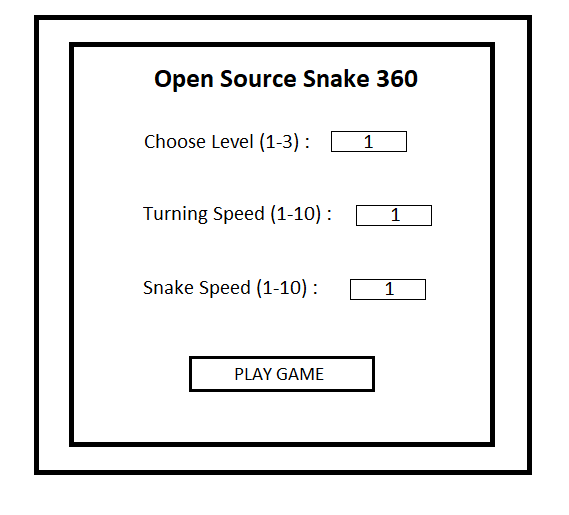
\includegraphics[scale=0.5]{menuUtama}  
	\caption[Rancangan tampilan menu utama]{Rancangan tampilan menu utama}
	\label{fig:menuUtama} 
\end{figure}

\begin{figure}[H]
	\centering  
	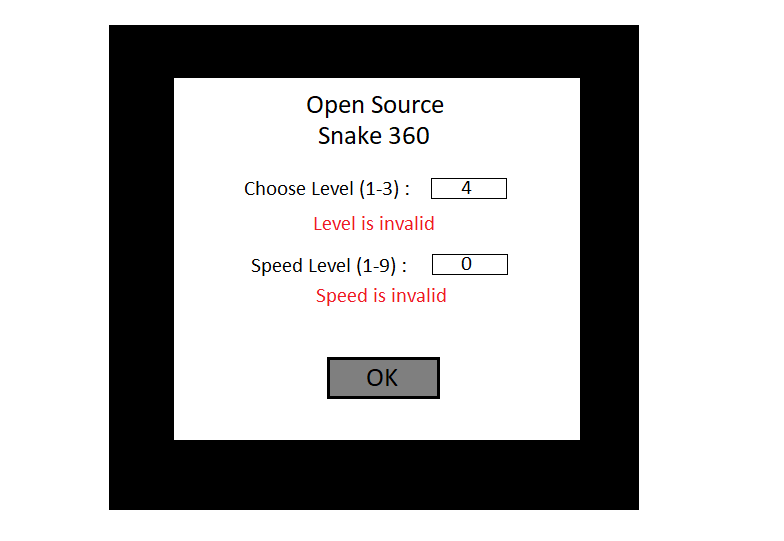
\includegraphics[scale=0.5]{menuUtamaSalah}  
	\caption[Rancangan tampilan menu utama jika pemain salah memasukkan data]{Rancangan tampilan menu utama jika pemain salah memasukkan data}
	\label{fig:menuUtamaSalah} 
\end{figure}

\subsection{Tampilan Bermain}
Tampilan bermain akan muncul setelah pemain memilih labirin, kecepatan ular dan kecepatan ular berbelok pada menu utama dengan benar dan sudah menekan tombol '\textit{Play Game}' (Gambar~\ref{fig:menuUtama}). Gambar~\ref{fig:permainan} merupakan tampilan permainan sudah dimulai. Pada tampilan ini terdapat ular, dinding labirin dan makanan berbentuk apel. Pada tampilan ini juga terdapat labirin yang dipilih dan skor yang didapat. 

\begin{figure}[H]
	\centering  
	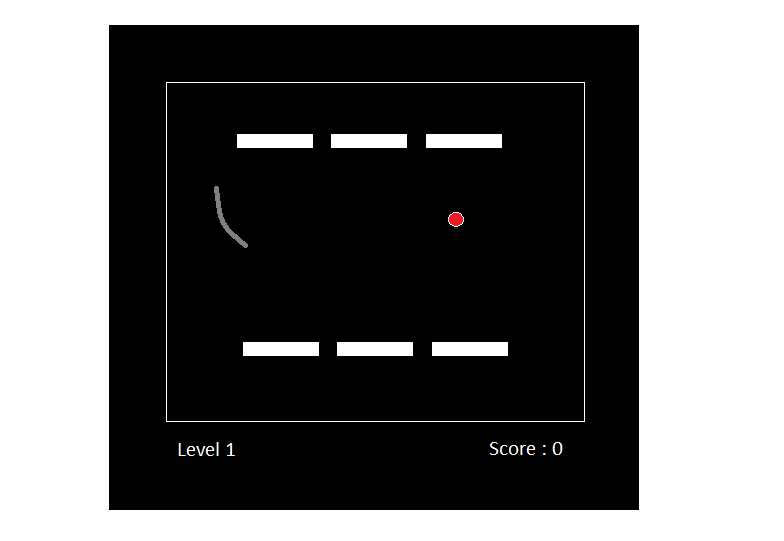
\includegraphics[scale=0.5]{permainan}  
	\caption[Rancangan tampilan bermain]{Rancangan tampilan bermain}
	\label{fig:permainan} 
\end{figure}

\subsection{Tampilan Permainan Berakhir}
Tampilan ini akan muncul apabila permainan berakhir. Permainan akan berakhir jika ular menabrak dinding labirin atau menabrak tubuhnya sendiri. Gambar~\ref{fig:permainanBerakhir} merupakan tampilan permainan berakhir. Pada tampilan ini, pemain dapat mengulang permainan dengan menekan tombol '\textit{Enter}'. Pemain akan dialihkan ke tampilan menu utama(Gambar~\ref{fig:menuUtama}) apabila tombol '\textit{Enter}' ditekan.

\begin{figure}[H]
	\centering  
	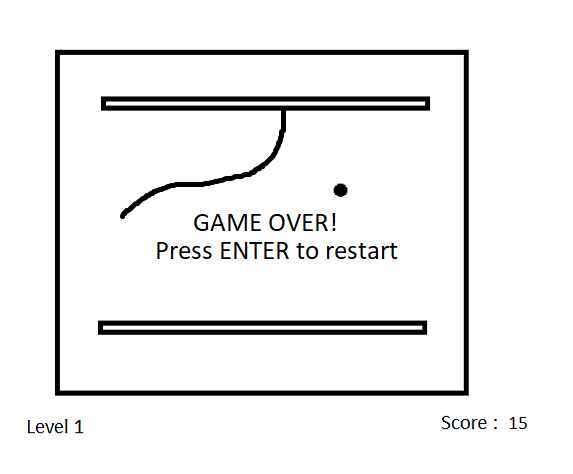
\includegraphics[scale=0.5]{permainanBerakhir}  
	\caption[Rancangan tampilan permainan berakhir]{Rancangan tampilan permainan berakhir}
	\label{fig:permainanBerakhir} 
\end{figure}